\documentclass[letterpaper,10pt]{article}

\usepackage{enumitem}
\usepackage{titling}
\usepackage{listings,listings-rust}
\usepackage{url}
\usepackage{soul}
\usepackage{hyperref}
\usepackage{setspace}
\usepackage{subfig}
\usepackage{sectsty}
\usepackage{pdfpages}
\usepackage{colortbl}
\usepackage{multirow}
\usepackage{multicol}
\usepackage{relsize}
\usepackage{amsmath}
\usepackage{wasysym}
\usepackage{fancyvrb}
\usepackage[yyyymmdd]{datetime}
\usepackage{amsmath,amssymb,amsthm,graphicx,xspace}
\usepackage[titlenotnumbered,noend,noline]{algorithm2e}
\usepackage[compact]{titlesec}
\usepackage{XCharter}
\usepackage[T1]{fontenc}
\usepackage[scaled]{beramono}
\usepackage[normalem]{ulem}
\usepackage{booktabs}
\usepackage{tikz}
\usetikzlibrary{arrows.meta,automata,shapes,trees,matrix,chains,scopes,positioning,calc,decorations.pathreplacing}
\tikzstyle{block} = [rectangle, draw, fill=blue!20, 
    text width=2.5em, text centered, rounded corners, minimum height=2em]
\tikzstyle{bw} = [rectangle, draw, fill=blue!20, 
    text width=4em, text centered, rounded corners, minimum height=2em]

\definecolor{namerow}{cmyk}{.40,.40,.40,.40}
\definecolor{namecol}{cmyk}{.40,.40,.40,.40}
\renewcommand{\dateseparator}{-}

\let\LaTeXtitle\title
\renewcommand{\title}[1]{\LaTeXtitle{\textsf{#1}}}

\lstset{basicstyle=\footnotesize\ttfamily,breaklines=true}

\newcommand{\CPP}{C\nolinebreak\hspace{-.05em}\raisebox{.4ex}{\tiny\bf +}\nolinebreak\hspace{-.10em}\raisebox{.4ex}{\tiny\bf +}}
\def\CPP{{C\nolinebreak[4]\hspace{-.05em}\raisebox{.4ex}{\tiny\bf ++}}}

\newcommand{\handout}[5]{
  \noindent
  \begin{center}
  \framebox{
    \vbox{
      \hbox to 5.78in { {\bf ECE459: Programming for Performance } \hfill #2 }
      \vspace{4mm}
      \hbox to 5.78in { {\Large \hfill #4  \hfill} }
      \vspace{2mm}
      \hbox to 5.78in { {\em #3 \hfill \today} }
    }
  }
  \end{center}
  \vspace*{4mm}
}

\newcommand{\lecture}[3]{\handout{#1}{#2}{#3}{Lecture#1}}
\newcommand{\tuple}[1]{\ensuremath{\left\langle #1 \right\rangle}\xspace}

\addtolength{\oddsidemargin}{-1.000in}
\addtolength{\evensidemargin}{-0.500in}
\addtolength{\textwidth}{2.0in}
\addtolength{\topmargin}{-1.000in}
\addtolength{\textheight}{1.75in}
\addtolength{\parskip}{\baselineskip}
\setlength{\parindent}{0in}
\renewcommand{\baselinestretch}{1.5}
\newcommand{\term}{Winter 2020}

\singlespace


\begin{document}

\lecture{20 --- Self-Optimizing Software}{\term}{Jeff Zarnett}

\section*{Self-Optimizing Software}
Our previous discussion about compiler optimizations (and optimizing the compiler) was focused on things that the compiler can do at compile-time. But what about runtime? The compiler can't do much at runtime, but a sufficiently-smart program can change itself at runtime to be better. Better, in this case, meaning faster. But what about change? We'll start with the simple things, and move on to the more complex  and harder to get right. The simple stuff has to do with changing what's in memory, and well advance into changing the configuration, and finally, we'll consider changing the binary itself.

\paragraph{Caching.} Your first thought about how a program might change itself for speed might be something like caching! Suppose that you keep track of the most popular exchange rates in memory, so that they are available faster than by going to the database. The management of the cache will be at runtime; the contents of the cache will be based on the actual usage. And, it will change over time to adapt to the patterns of usage: if today the exchange rate of CAD-EUR is popular, it will appear in the cache, and without any code changes if the exchange rate of CAD-GBP becomes popular, it goes in the cache and becomes faster to access. So, you \textit{do} technically get different behaviour at runtime, but this is not quite what we wanted to talk about in this topic. It's too easy, and your program should probably be doing it already.

\paragraph{Observe and change.}
The next idea relates to having your program's configuration change at runtime to adapt to observed behaviour. If there are multiple routes to the same outcome, we might decide at runtime which is the best. This is effective because our initial guess might not be correct, but also because conditions can change at any time.

If you've taken a course in databases, you should have been exposed to the idea of query processing: given a certain query (\texttt{SELECT id FROM... JOIN... WHERE...}), the database server comes up with an execution plan for how to carry it out. For a simple query, there might be only one answer. A more complex query will have multiple correct answers and the database server will do what it considers best. However, that is based on an estimated cost only. The server could, at least once, try out a different strategy and notice if it is better than the original plan. A lot of queries happen many times (or are extremely similar to already-observed queries), so remembering what worked is helpful.

Building on that, the database server could change how it organizes the data based on what would be most efficient for the most common usage patterns. You can do the same in your program. For an analogy, I can sort the Excel sheet with student grades by either student ID (20xxxxxx) or user ID, based on whatever I use more. So if it is during the term and I'm entering grades, I probably use student ID as the way the file is sorted so I can get efficiently where I need to go. And I could always change that organization if it makes sense, such as after the end of term when people may e-mail me (including their user ID, but not student ID). The idea of re-structuring data storage can also apply to files on disk.

The observe-and-change strategy can also apply when invoking external services (external as in, over the internet). Suppose there are three different servers where we can send messages and we'll measure and remember how long it took to get a response from that server. The fastest server might be the one that is the closest geographically, but that server might be very busy, so it might be faster to communicate with a server that's less busy but farther away. Maybe you send 8 out of every 10 messages to the server that was most recently determined to be the fastest, and one to each of the other two servers. You might discover that your current guess at the fastest server is wrong and it's better to switch your primary.


\paragraph{Genetic algorithms.}
If you've taken an advanced course on algorithms, you might have covered genetic algorithms in some detail. This isn't going to be a replacement for that, but will just give you an idea of how the idea can be used. First, a quick three-paragraph explainer on genetic algorithms~\cite{genetic}.

A genetic algorithm is inspired by the idea of natural selection. Our program is trying to solve a particular problem. A number of candidate solutions are created (usually, randomly) and they are evaluated for their fitness: how well do they solve the problem? Solutions with a higher fitness have a higher chance of continuing forward into the next group of candidates, called the next generation. At each generation, good solutions from the previous generation are combined (if possible) and/or mutated randomly to see if that makes the solution better. This process repeats until a sufficiently-optimal solution is found, or a fixed number of generations have been evaluated. Thus, solutions with good qualities ``reproduce'' and move forward in the simulation, and those with bad qualities ``die out'' and we do not continue down that path. If we do this well, eventually we end up with a solution that's good, or at least good enough.

This works for the kind of problem where we, first of all, have some parameters to configure. If there is nothing to configure, there's nothing to change or evolve. We also need a fitness function that allows us to evaluate how well the problem is being solved. This function cannot be binary (pass/fail) because that doesn't show whether a given solution A is better or worse than solution B; instead we want a continuous or discrete (in the mathematical sense) definition of fitness so we can say solution A with 84.1 is better than B with 81.0.

Of course, a genetic algorithm does not necessarily guarantee the best possible outcome. It is possible that the fitness function tends towards a local-maximum rather than the global one, so we get a good solution but not the best. Similarly, the fitness of a solution might be evaluated rarely or take a long time, making the process of finding a good solution slow.

Right, with that in mind, you might ask how genetic algorithms help in making your program faster. The typical use for a genetic algorithm is something like designing an antenna or an airplane wing where making random changes gives some numbers. We can do the same with a generic program, if it has the right properties and what we're trying to do is optimize our configuration parameters.

Let's return to the subject of Google Maps. In our earlier discussion on early-phase termination, we tried to brainstorm ideas about how potential routes are generated and how we know if we have enough or a good-enough route. In the discussion, we will imagine that the decision of when to terminate the search is based on when we have a ``good enough'' solution. Then there are the various parameters that go into generating a solution, which I'll guess to be something like:

\begin{itemize}
	\item Number of routes to evaluate
	\item Heuristic for generating routes to evaluate
	\item Decay of traffic information reported by other motorists
	\item Time of day and month and if it's a holiday
	\item Search radius for alternate routes
\end{itemize}

It is Google, after all, so they probably consider many more parameters or use a completely different mechanism. It might be very difficult to choose what the correct values for these parameters are (especially if they vary by time of day, day of the week, on holidays, etc). Changing them by hand probably does not work, but letting a genetic algorithm choose the values based on experimenting and trading off the quality of the solution against the time to come up with it. We might consider a solution that only comes up with awful routes to fail, even if it gets them nearly instantly. And we might consider the successful solution one that comes up with a route that is optimal or nearly-optimal in the shortest time.

One reason why genetic algorithms might be a good choice for this kind of problem is that the problem is nonlinear: that is, we cannot treat each parameter as an independent variable and change just one and expect that the change in output is only a result of the change of the one input variable and not also an interaction of one variable with others~\cite{genetic}.

Perhaps this takes away some of the mystery of genetic algorithms. Maybe you're thinking this isn't really self-optimizing software, it's just optimizing configuration parameters. Let's go up (well, really, down) a level, then. Now we'll move into changing the binary itself.

\paragraph{Hotspot.}
The previous discussion of compiler optimizations talked about all the things that compiler can do to make the program more efficient. Some of them are always a clear win. Precomputing something or skipping unnecessary code is always going to be better than the alternative. Other optimizations are not. Let's consider the decision about inlining: sometimes it's good, but sometimes it doesn't help or makes things worse. In those cases, the compiler has to take a decision about whether to do it or not and that's what is in the binary.

In JVM-languages like Java, the virtual machine itself can do some optimization because of the just-in-time (JIT) compiler. The original program is turned into the intermediate representation by the Java compiler, and then there's a second chance at runtime! Oracle's documentation tell us that there's actually two different JIT compilers; one for clients and one for servers. The client one produces its output faster, but that code produced will be less efficient. The server one takes more time and more resources to produce slightly better code.

The major advantage that the JIT compiler has is being able to observe the runtime behaviour of the program and then change its decision. If we see that, for example, inlining would be helpful but the original decision was not to do it, we can change that decision. This is very helpful in scenarios like inlining, because we'll have the function call overhead every single time and therefore every call to the function increases the penalty of getting the decision wrong. Being able to change our decision is less helpful when it comes to something like a branch prediction, because the hardware will most likely save us if our prediction isn't very good (see our earlier discussion on this topic).

There are actually a few other things that can be done by the JIT compiler at runtime which are not likely to be doable at compile time. In particular, I want to focus on \textit{escape analysis} \textit{on-stack replacement}, and \textit{intrinsics} as outlined in~\cite{escape}.

Let's start with escape analysis. The purpose of this is to figure out if there are any side effects visible outside of a particular method. This allows some skipping of heap allocation and we can stack allocate them instead. The more interesting thing are possible lock optimizations: lock elision, lock coarsening, and nested locking. Lock elision: if the JIT compiler can determine that a lock serves no purpose -- e.g., a method or block is tagged as \texttt{synchronized} but it can only ever get called from one thread at a time -- there's no lock at all and therefore no setup an1d acquisition costs.  Lock coarsening: if there are sequential blocks sharing the same lock, the compiler can combine them to reduce the amount of locking and unlocking that needs to happen. The cuts down the overhead and we'll take it where we can. Nested locks: if the same lock is required repeatedly without releasing (in some recursive code, perhaps) this can also be combined so we don't have as much overhead lost to locking and unlocking.

On-stack replacement is a way that the virtual machine can switch between implementations of a particular method. This is helpful if a function is identified as important (sometimes called \textit{hot}) in that it runs frequently, then a more optimized version can be swapped in. This does have a slight cost, in that the virtual machine has to pause execution briefly to swap in the new stack frame (as it may be organized a differently), but it will be of some benefit in the long run if this function is truly a frequently-executed piece of code.

If you've done debugging in a JVM language like Java or Kotlin you might have seen something like this in action! While you have the debugger attached, you can make changes, compile it, and the JVM will try to swap in the new code for the old code and continue running. This does not always succeed, but if it does it allows you to try a changed version of the program without having to stop and restart. That's particularly helpful when there's a long workflow to reproduce a particular problem and/or the application in question takes a long time to start up.

Intrinsics are highly-optimized versions of code that is precompiled for a specific platform (e.g., x86). If a particular piece of code is truly critical, then using that native implementation might be faster, but it might not always be available, depending on your platform. These were originally developed in \CPP~rather than Java so it's also done without the safety rails of Java. I guess in that sense you could say that \CPP~ is Java's unsafe mode. That might be a controversial statement. Now there's a different approach called Graal, which turns the Java bytecode directly into machine code. Adding an intrinsic is a complicated process.

The hotspot approach is probably closest to what you might have imagined by reading the title of this topic: changing the binary code based on observed runtime behaviour of the program. Rust doesn't have the capability of detecting the parameters at runtime and swapping binary code them, because it has chosen not to have a runtime like the JVM. While that does mean that there's less overhead in general, the tradeoff is that any decisions made at compile time will remain so. Unless...

\paragraph{Rewriting the binary.}
Rewriting the binary in a language like C or Rust can happen, but requires us to do more work ourselves, or depend on a library that implements that functionality for us.

One possibility is to have different versions of a compiled block of code at the ready. That is, we direct the compiler, when the program is being built, to make several variants of the same code with different optimization decisions or other tradeoffs. We'll start with a default, and if we determine based on some observation that we need to change, then overwrite that part of the binary in memory with the new version and we've changed the code path that executes!

There are a couple difficulties that that approach, though. Yes, it increases compile time, but that's usually acceptable as a tradeoff, and is of minor concern. The first big question is how many variants of the code will you compile and have prepared? This is still compile-time work so we're not sure what the real data and behaviour will be like at runtime, so we are still guessing, but we get multiple guesses instead of just one. Then we have to make sure a section of code isn't being executed when we want swap it out, but that's possible to do with some locking mechanism or other software coordination.

That approach is rewriting the binary at run-time, but you might be thinking that if it's all precompiled anyway, can't we decide at runtime with if-statements what function to call to get the same effect? I think so, and thus we haven't really reached the real goal which is doing it truly dynamically. Which is an option.

So, you want to compile your own code. With our understanding of all the things the compiler does, you can reasonably assume that you're not going to write your own and include it in your program. Code generation isn't magic or so incredibly difficult that you can't do it, but if you want to make optimal code you need a lot of the analytics and decision-making that's in the compiler. So the only realistic way of getting the code compiled is to use an existing compiler, that is, the one that's already on the target system.

Requiring a specific compiler on the target system might limit your ability to actually deploy this technique. For one thing, if it's end-user software, they might not have compilers installed at all (Windows?), or if they do it's a different compiler (LLVM vs gcc, perhaps)? And you might also encounter a security policy on your servers that forbids the installation of a compiler to make it harder for any exploit that somehow works its way in to compile and run its payload.

If we can actually use the compiler on the target system, then we are in business. The approach is simple to explain if somewhat complicated in practice. First, take the binary code of the segment that we want to optimize and then have the compiler take a look at it. The compiler will then take the binary, convert it to its internal representation (the intermediate representation), then optimize it, and compile it. The new binary code can get swapped in when it's ready.

On top of the advantage of having runtime information when compiling this time, this kind of approach makes it possible to inline or rewrite library functions if we want too. The amount of benefit will vary a lot based on the library. Some are pretty efficient as-is, but others with lots of functionality might benefit a lot by being optimized for the one use-case you need.

Does this work? Yes; here's some research on the subject from~\cite{binaryrewriting}. They are doing a calculation on a matrix of size 649 $\times$ 649 for 20~000 iterations. Here's their graph of the performance results from the improved code:

\begin{center}
	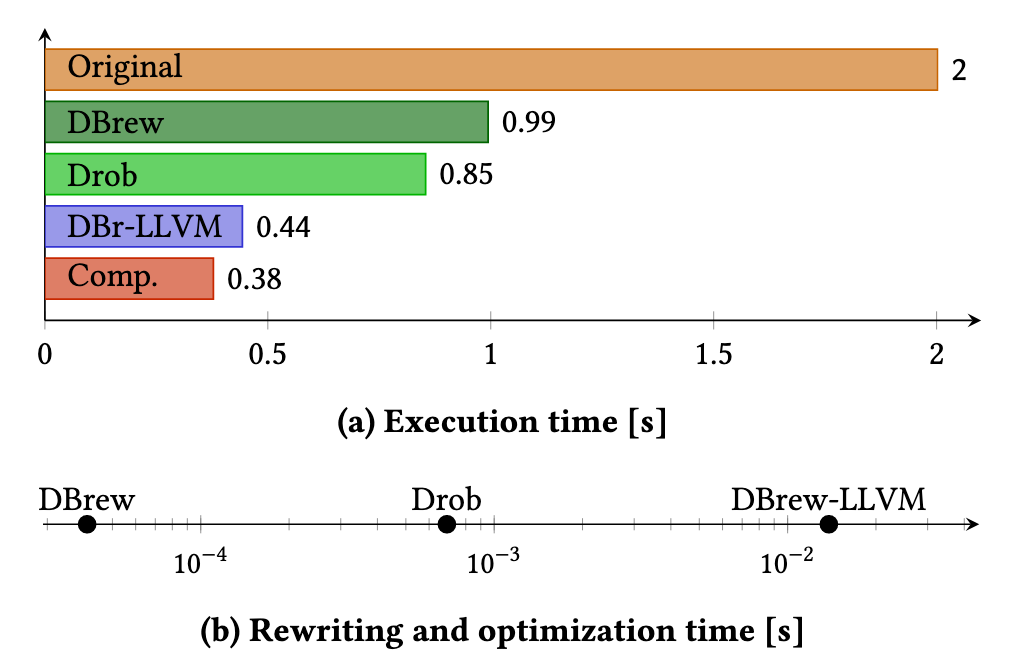
\includegraphics[width=0.6\textwidth]{images/rewriting.png}
\end{center}

As expected, there is a significant cost associated with the process of recompiling a segment of the program. But given the right workload, there is clearly a benefit in the execution time of the updated program. In that case, this is worth doing on code that will run frequently.

\paragraph{Program sus.}
It's worth noting that programs that rewrite themselves are frequently judged as suspicious by anti-virus and anti-malware software. The story behind this is a part of a software arms race. It starts with the first viruses, which are malicious code doing malicious things. So, anti-virus software is developed to detect viruses and the primary mechanism for detecting if something is a virus is comparing the binary code under examination against a database of malicious software.

To combat this binary-matching pattern, some viruses will alter themselves in subtle ways or produce code that's functionally equivalent but looks different in binary than the original. A virus is not usually something that requires excellent performance, so making a transformation that's slower but looks different to the virus scanner is fine (from the villain point of view, anyway).

It's impossible to predict all possible transformations for a particular piece of software, because there's a lot of routes to the same destination. Anti-virus software can try to ignore things like inserted NOPs or pay no attention to variables X and Y being swapped and then swapped back to just add some assembly instructions. Still, an alternative approach that some anti-virus programs choose is heuristic analysis, which is analyzing broadly what the program under examination does and seeing if its behaviour looks... suspicious.

Combining those two facts means that a benign program that changes its own binary code might be considered by anti-virus software to be suspicious and prevented from running or otherwise restricted in some way. If you're determined to rewrite the binary, just keep in mind that anti-malware software end-users have installed may affect the experience (if you are, in fact, shipping to end-users at all).
\bibliographystyle{alphaurl}
\bibliography{459}


\end{document}
